\documentclass[11pt]{article}
% Workshop version (4 pages + references + appendix). Same numbers, figures and bibliography as main.tex,
% the full arXiv version; every number comes from numbers.json or a commit-pinned journal entry.

\usepackage[margin=1in]{geometry}
\usepackage[T1]{fontenc}
\usepackage{amsmath,amsthm}
\usepackage{newtxtext,newtxmath}
\usepackage{microtype}
\setlength{\emergencystretch}{2em}
\usepackage{booktabs}
\usepackage{float}
\usepackage{graphicx}
\usepackage{xcolor}
\usepackage{enumitem}
\usepackage[font=small,labelfont=bf]{caption}
\usepackage{subcaption}
\usepackage[numbers,sort&compress]{natbib}
\usepackage[colorlinks=true,linkcolor=blue!60!black,citecolor=blue!60!black,urlcolor=blue!60!black]{hyperref}

\newtheorem{proposition}{Proposition}
\newcommand{\pending}[1]{\textcolor{red!70!black}{[\textsc{pending}: #1]}}
\newcommand{\tree}{\textsc{tree}}
\newcommand{\vis}{\textsc{vision}}
\newcommand{\fb}{\textsc{fallback}}

\makeatletter
\renewcommand{\maketitle}{\begin{center}
  {\Large\bfseries Tree First, Else Vision Is Worse Than Vision:\\[3pt]
   When to Trust the Accessibility Tree in GUI Grounding\par}\vspace{8pt}
  {\large Rudra Naresh}\\[2pt]
  {\small\texttt{[affiliation]} \quad \texttt{[email]}}
\end{center}\vspace{2pt}}
\makeatother

\begin{document}
\maketitle

\begin{abstract}
Computer-use agents often ground an instruction by asking the accessibility tree first and falling back
to a vision model when the tree has no answer. We measure this policy with ground truth that comes from
neither source. On generated pages covering five ways a tree can fail, and on real Windows screens whose
trees we damage on purpose, the tree-first policy is less accurate than vision alone ($-12.0$ and $-9.5$
points). The loss equals the tree's answer rate times the gap between its precision and vision's accuracy on
the items it answers: the tree keeps answering on ambiguous and canvas-drawn targets, and is then right 54\%
of the time where vision is right 80\%. A gate that trusts an LLM's reading of the tree only when the chosen
element has a name reaches 85.2\% against 66.4\% for vision, and is never below vision on any condition. The
vision side is a 2B grounder trained on 1,572 examples labelled for free by Windows UI Automation on one T4
GPU, which raises accuracy on unseen applications from 1.5\% to 46.5\%.
\end{abstract}

\section{Introduction}

Grounding maps a description such as ``click Save'' to a point on the screen. The accessibility tree (UI
Automation on Windows, the DOM accessibility tree in browsers) lists elements with names and boxes, and is
exact when it contains and names the target. It often does not: 29.6\% of the top million web home pages
have a button with no accessible name~\citep{webaim2025}, and canvas content (spreadsheet grids, CAD
viewports, whiteboards) is absent from it. Agent systems therefore combine the tree with vision; UFO2 merges
UI Automation with a vision parser~\citep{zhang2025ufo2}, and production browser agents read the
accessibility snapshot first and request a screenshot only when an element is missing~\citep{vardanyan2025browser}.

This tree-first policy is safe only if the tree abstains whenever it cannot resolve the target. A name
matcher does not: asked for an unnamed target it returns the element with the closest name, and given two
buttons named ``Archive'' it returns the first. Vision grounders~\citep{cheng2024seeclick,lin2025showui,gou2025uground,wu2025osatlas}
and recent work on their calibration~\citep{wang2026safeground,zhang2025hyperclick} ask when to trust the
grounder; we ask when to trust the tree.

\paragraph{Contributions.} (1) A per-condition comparison of tree, vision and hybrid policies with ground
truth independent of both, on generated pages and on real Windows trees; (2) an exact decomposition of the
tree-first loss, which also predicts the gain of any gate; (3) a gate based on whether the chosen element has
a name, chosen on dev and tested once; (4) a 2B UIA-supervised grounder trained on free hardware.

\begin{figure}[t]
\centering
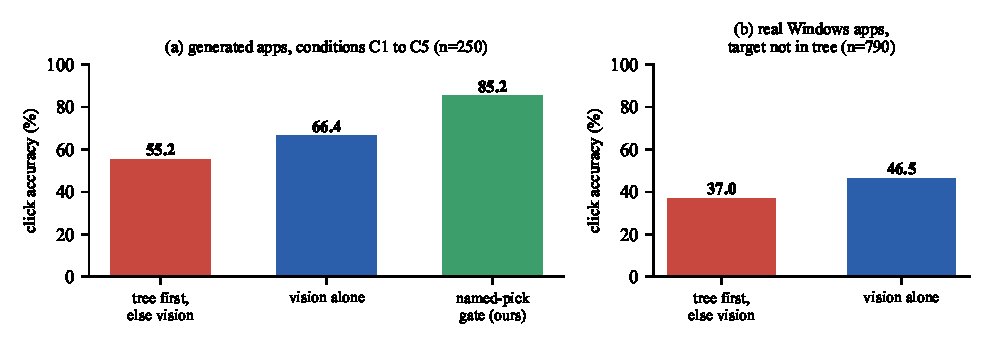
\includegraphics[width=0.9\linewidth]{figures/teaser.pdf}
\caption{Click accuracy (\%). (a) Generated pages, the same 250 items for all three policies. (b) Real
Windows applications (four never trained on) with the target missing from the tree.}
\label{fig:teaser}
\end{figure}

\section{Setup}

An item is a screenshot, an instruction $q$ and a target box; a point \emph{hits} if it lies in the box,
and the same rule scores every method. Five conditions relate $q$ to the tree $T$: \textbf{C1} the target
is named as $q$ names it; \textbf{C2} it is in $T$ without a name; \textbf{C3} $q$ paraphrases its name;
\textbf{C4} it is drawn on a canvas and absent from $T$; \textbf{C5} several elements share its name and
$q$ disambiguates by context. Policies: \tree{} (fuzzy name matching, ties to the first in tree order);
\vis{} (the grounder's point); \fb{} (\tree{} if it answers, else \vis); \textsc{tree\_llm} (an LLM reads
$T$ and answers one element or NONE); \textsc{llm\_guarded} (its pick, else \vis); \textsc{llm\_named} (its
pick only if the element has a name, else \vis).

\begin{proposition}
\label{prop:decomp}
Let $A$ be the event that the tree answers, and $h_r$, $h_g$ the hit indicators of the tree's and the
grounder's points. Then $\mathrm{Acc}(\fb) - \mathrm{Acc}(\vis) = \Pr(A)\,(\Pr(h_r\mid A) - \Pr(h_g \mid A))$.
More generally, a policy that uses the tree on a subset $S$ and the grounder elsewhere gains
$\Pr(S)\,(\Pr(h_r\mid S) - \Pr(h_g\mid S))$ over \vis.
\end{proposition}
The proof is one line: the policies agree outside $S$. The quantity to measure is therefore not the tree's
accuracy but its answer rate and its precision on the items it answers, against vision on those items.

\paragraph{Grounder.} Qwen2-VL-2B~\citep{wang2024qwen2vl} with LoRA~\citep{hu2022lora} ($r{=}16$), trained
on 1,572 targets that Windows UI Automation names and boxes for free (10 apps), three epochs on one Kaggle
T4 (8\,h). The checkpoint was chosen on dev and pushed before any test item was scored; intervals are
paired bootstrap 95\% CIs resampled by screenshot. On four unseen apps (790 targets) accuracy rises from 1.5
to 46.5 ($+44.9$ [41.1, 48.7]); on ScreenSpot-v2 from 19.2 to 62.8 ($+46.1$ [42.9, 49.1]).

\section{Results}

\paragraph{Test A: generated pages.} True boxes come from the DOM or canvas geometry. The frozen test set
has 1,000 items, 200 per condition (Table~\ref{tab:a}). The tree wins only C1. \fb{} loses 12.0 points
[9.7, 14.4] to vision, and the decomposition locates the loss: the tree answers every C5 item and a quarter
of C4 items, and overrides a correct vision click on 49.5\% and 23.5\% of them.

\begin{table}[t]
\centering\small
\begin{tabular}{lcccccc}
\toprule
& C1 & C2 & C3 & C4 & C5 & all \\
\midrule
\tree{} accuracy & \textbf{100.0} & 0.0 & 0.0 & 0.0 & 26.5 & 25.3 \\
\vis{} accuracy & 94.0 & \textbf{40.0} & \textbf{31.0} & \textbf{99.0} & \textbf{65.0} & \textbf{65.8} \\
\fb{} accuracy & 100.0 & 37.5 & 29.5 & 75.5 & 26.5 & 53.8 \\
\midrule
tree answers, $\Pr(A)$ & 100.0 & 4.5 & 6.0 & 23.5 & 100.0 & 46.8 \\
tree precision on $A$ & 100.0 & 0.0 & 0.0 & 0.0 & 26.5 & 54.1 \\
vision accuracy on $A$ & 94.0 & 55.6 & 25.0 & 100.0 & 65.0 & 79.7 \\
\fb{} $-$ \vis{} & $+6.0$ & $-2.5$ & $-1.5$ & $-23.5$ & $-38.5$ & $-12.0$ \\
\bottomrule
\end{tabular}
\caption{Test A (\%, 200 items per condition) and the decomposition of Proposition~\ref{prop:decomp}.}
\label{tab:a}
\end{table}

\paragraph{Test B: real Windows trees, damaged on purpose.} The grounder never reads the tree, so its saved
answers on real test screenshots can be re-scored against the real UI Automation tree with the target's name
blanked or the target removed. On the unseen apps, \vis{} is 46.5 in every state and \fb{} falls to 37.0
when the tree lacks the target ($-9.5$ [$-11.8$, $-7.4$]): the tree still answers on 25.8\% of items,
through another element with a similar name, and is right on 3.9\% of those against 40.7\% for vision,
which gives $0.258 \times (3.9 - 40.7) = -9.5$. With the tree intact, \fb{} reaches 93.0, so the tree is
valuable when it has the target; the problem is knowing when it does.

\paragraph{Gates.} On the first 50 test pages (250 items, fixed in advance), an LLM reading the tree
(gpt-oss-120b) fixes rewording and ambiguity (C3 88, C5 100) but not blindness (C2 2, C4 0)
(Table~\ref{tab:gates}). The pre-registered \textsc{llm\_guarded} reaches 83.2 but loses 6 points to vision
on unnamed icons, where the LLM picks an element instead of answering NONE. Among four repairs frozen before
any dev answer, \textsc{llm\_named} was chosen on 300 new dev items and scored once: 85.2, $+18.8$
[15.2, 22.4] over vision. The proposition explains why: the LLM's named picks (59.2\% of items) are 93.2\%
precise where vision is 61.5\% on the same items, and $0.592 \times (93.2 - 61.5) = +18.8$, the measured
gain. Its nameless picks (4.0\%) are 10\% precise where vision is 60\%, so excluding them is correct.

\begin{table}[t]
\centering\small
\begin{tabular}{lcccccc}
\toprule
policy (same 250 items) & C1 & C2 & C3 & C4 & C5 & mean \\
\midrule
\fb & & & & & & 55.2 \\
\vis & 98 & 38 & 28 & 100 & 68 & 66.4 \\
\textsc{tree\_llm} & 88 & 2 & 88 & 0 & 100 & 55.6 \\
\textsc{llm\_guarded} (pre-registered) & 92 & 32 & 92 & 100 & 100 & 83.2 \\
\textbf{\textsc{llm\_named}} (chosen on dev) & 94 & 38 & 94 & 100 & 100 & \textbf{85.2} \\
\bottomrule
\end{tabular}
\caption{Gates on the 250-item subset of Test A (\%). \textsc{llm\_named} is never below vision.}
\label{tab:gates}
\end{table}

\paragraph{In an agent.} The decision-making LLM of an agent already reads the tree, so the gate costs no
extra call. We enforce it in a perceive, decide, ground, act and verify loop: the LLM returns one intent
naming an element or describing a target; a router accepts element ids only for named elements, sends
descriptions to the grounder, and refuses bare click coordinates; task success is read from application
state. \pending{task-level results on five sandbox tasks, one per condition.}

\section{Limitations and conclusion}

Test A is synthetic and Test B's stored tree holds only named elements, so it is cleaner than a live tree;
the gate was confirmed on 250 synthetic items; four unseen apps and one training seed
\pending{second seed}. The grounder is trained only on named elements, yet its role is the nameless and the
absent \pending{Test C: real targets the tree cannot see}. Within these limits the result is consistent across
both test beds: a tree-first merge is less accurate than vision alone once the tree is incomplete, its loss is
the tree's answer rate times its precision gap, and a gate that trusts only named tree picks recovers the
tree's advantage without the loss.

\bibliographystyle{plainnat}
\bibliography{refs}

\appendix
\section{Additional results}

\begin{figure}[H]
\centering
\begin{subfigure}{0.49\linewidth}\centering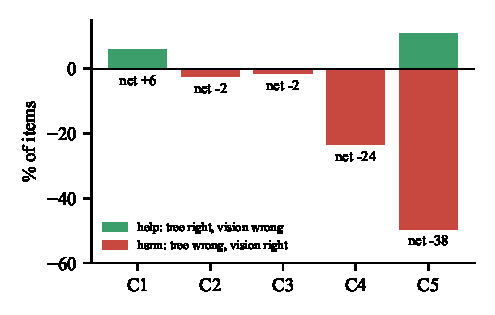
\includegraphics[width=\linewidth]{figures/test_a_help_harm.pdf}
\caption{Test A: help and harm of \fb.}\end{subfigure}
\begin{subfigure}{0.49\linewidth}\centering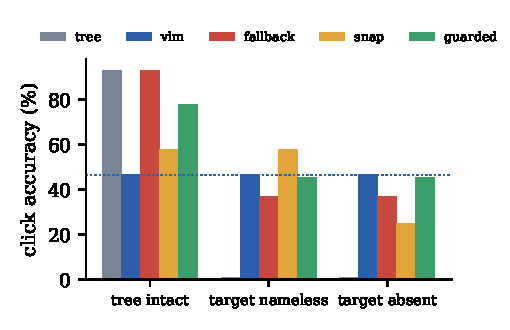
\includegraphics[width=\linewidth]{figures/test_b.pdf}
\caption{Test B: unseen apps, three tree states.}\end{subfigure}
\caption{(a) The tree-first loss is harm (tree wrong, vision right), concentrated on C4 and C5. (b) Real
screens: \fb{} and snapping fall below vision once the target is missing; the exact-name guard does not.}
\end{figure}

\begin{table}[H]
\centering\small
\begin{tabular}{lccc}
\toprule
& zero-shot & fine-tuned & $\Delta$ [95\% CI, screenshot-clustered] \\
\midrule
same apps, new screenshots ($n{=}246$) & 14.2 & 64.6 & $+50.4$ [43.0, 57.8] \\
four unseen apps ($n{=}790$) & 1.5 & 46.5 & $+44.9$ [41.1, 48.7] \\
ScreenSpot-v2, 6-cell mean ($n{=}1{,}272$) & 19.2 & 62.8 & $+46.1$ [42.9, 49.1] \\
\bottomrule
\end{tabular}
\caption{The grounder. Full training and evaluation details, the failure log, and the agent are in the
full version.}
\end{table}

\end{document}
